\let\negmedspace\undefined
\let\negthickspace\undefined
\documentclass[journal]{IEEEtran}
\usepackage[a5paper, margin=10mm, onecolumn]{geometry}
%\usepackage{lmodern} % Ensure lmodern is loaded for pdflatex
\usepackage{tfrupee} % Include tfrupee package

\setlength{\headheight}{1cm} % Set the height of the header box
\setlength{\headsep}{0mm}     % Set the distance between the header box and the top of the text

\usepackage{gvv-book}
\usepackage{gvv}
\usepackage{cite}
\usepackage{amsmath,amssymb,amsfonts,amsthm}
\usepackage{algorithmic}
\usepackage{graphicx}
\usepackage{textcomp}
\usepackage{xcolor}
\usepackage{txfonts}
\usepackage{listings}
\usepackage{enumitem}
\usepackage{mathtools}
\usepackage{gensymb}
\usepackage{comment}
\usepackage[breaklinks=true]{hyperref}
\usepackage{tkz-euclide} 
\usepackage{listings}
% \usepackage{gvv}                                        
\def\inputGnumericTable{}                                 
\usepackage[latin1]{inputenc}                                
\usepackage{color}                                            
\usepackage{array}                                            
\usepackage{longtable}                                       
\usepackage{calc}                                             
\usepackage{multirow}                                         
\usepackage{hhline}                                           
\usepackage{ifthen}                                           
\usepackage{lscape}
\begin{document}

\bibliographystyle{IEEEtran}
\vspace{3cm}

\title{CHAPTER - 9\\Differential Equations}
\author{EE24BTECH11061 - Rohith Sai}
% \maketitle
% \newpage
% \bigskip
{\let\newpage\relax\maketitle}

\renewcommand{\thefigure}{\theenumi}
\renewcommand{\thetable}{\theenumi}
\setlength{\intextsep}{10pt} % Space between text and floats

\numberwithin{figure}{enumi}
\renewcommand{\thetable}{\theenumi}

\section*{Exercise : 9.6}
\begin{enumerate}
\item [12)] Solve the differential equation $\brak{x + 3y^2} \frac{dy}{dx} = y $ \\
\textbf{Solution (using the Method of Finite Differences):}\\
The given differential equation is:
\begin{align}
    \brak{x + 3y^2}  \frac{dy}{dx} &= y 
\end{align}

Rearranging the equation to express $\frac{dx}{dy}$ for Euler's method:
\begin{align}
    \frac{dx}{dy} &= \frac{x + 3y^2}{y}
\end{align}

Using the method of finite differences, the next value of $x$ can be computed as:
\begin{align}
    x_{n+1} &= x_n + h \cdot f\brak{y_n, x_n} \\
    f\brak{y, x} &= \frac{x + 3y^2}{y}
\end{align}

Let $y_0$ be the initial $y$ value and $x_0$ be the initial $x$ value. Let the step size $h$ be 0.001. The first few iterations are:

\begin{align*}
y_1 &= y_0 + h, & x_1 &= x_0 + h \cdot \frac{x_0 + 3y_0^2}{y_0} \\
y_2 &= y_1 + h, & x_2 &= x_1 + h \cdot \frac{x_1 + 3y_1^2}{y_1} \\
&\vdots  & \vdots \\
y_n &= y_{n-1} + h, & x_n &= x_{n-1} + h \cdot \frac{x_{n-1} + 3y_{n-1}^2}{y_{n-1}}
\end{align*}

\textbf{Solution (using the general method):}\\
From equation (2), 
\begin{align}
    \frac{dx}{dy} = \frac{x+3y^2}{y}\\
    \implies \frac{dx}{dy} - \frac{x}{y} = 3y
\end{align}
On comparing equation (6) with the standard form of differential equation 
\begin{align}
    \frac{dx}{dy} + Px = Q
\end{align}
we get\\
$P = -\frac{1}{y}$ and $Q = 3y$.\\
Now we find the Integrating Factor (I.F.) in the following manner:
\begin{align}
    \text{I.F. } = \,e^{\int P \,dy}\\
    \implies \text{I.F. } = \,e^{\int -\frac{1}{y}\, dy}\\
    \implies \text{I.F. } = \,\frac{1}{y}
\end{align}
Therefore, solution is
\begin{align}
    x \cdot \brak{\text{I.F.}} = \int Q \cdot \brak{\text{I.F.}}  \,dy + C
\end{align}
On substituting the value of I.F. in equation (11) and solving, we get:
\begin{align}
    x = 3y^2 + Cy
\end{align}
Let's assume $C = -2$ and $y=1$. On substituting these values in equation (12), we get $x = 1$.\\
Therefore, the equation is
\begin{align*}
    x = 3y^2 - 2y
\end{align*}
Therefore, the curve generated using both the above mentioned methods for the given differential equation (1) is shown below:
\begin{figure}[H]
    \centering
    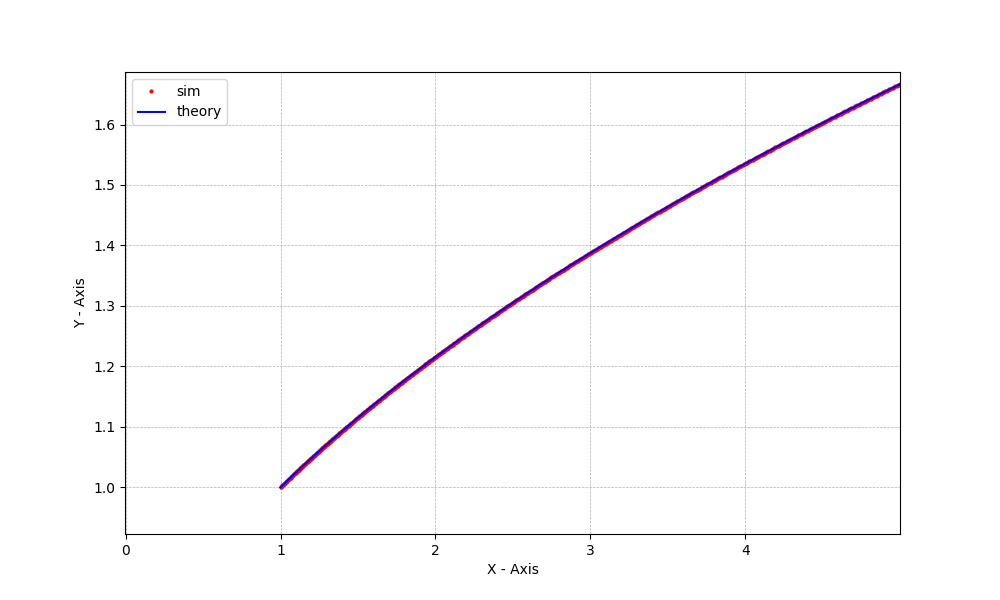
\includegraphics[width = \columnwidth]{figs/fig.png}
\end{figure}
\end{enumerate}
\end{document}